%-------------------------------------------------------------------------------
%-------------------------------------------------------------------------------
%-------------------------------------------------------------------------------
\chapter{Instructions conditionnelles}
%-------------------------------------------------------------------------------
%-------------------------------------------------------------------------------
\thispagestyle{empty}
%-------------------------------------------------------------------------------
%-------------------------------------------------------------------------------
\begin{abstract} Dans ce T.P. nous allons utiliser les instructions conditionnelles \type{if, else, elif}. Elles permettent d'adapter le traitement des données selon les cas.
\end{abstract}
%------------------------------------------------------------
%-------------------------------------------------------------------------------
%-------------------------------------------------------------------------------
\section{Exercices}
%-------------------------------------------------------------------------------
%-------------------------------------------------------------------------------
%------------------------------------------------------------
\begin{Exercise}Écrire une fonction \type{seuil(x)} telle que
$\displaystyle\text{seuil}(x) = \left\{\begin{matrix} 0&\text{ pour }x \le 0\\
x&\text{ pour }0\le x \le 1\\
1&\text{ pour }1\le x 
\end{matrix}
\right.$
\begin{center}
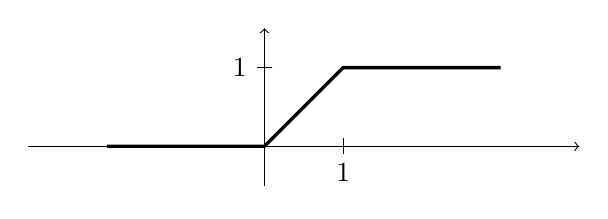
\begin{tikzpicture}
\draw[->] (-3, 0) -- (4, 0);
\draw[->] (0, -0.5) -- (0, 1.5);
\draw (1, 0.1) -- (1, -0.1) node[below] {1};
\draw (0.1, 1) -- (-0.1, 1) node[left] {1};
\draw[very thick] (-2, 0) -- (0, 0) -- (1, 1) -- (3, 1);
\end{tikzpicture}
\end{center}
\end{Exercise}
%-------------------------------------------------------------------------------
\begin{Answer}
\begin{lstlisting}
def seuil(x):
    if x < 0:
        return 0
    elif x < 1:
        return x
    else:
        return 1
\end{lstlisting}
\end{Answer}
%-------------------------------------------------------------------------------
%-------------------------------------------------------------------------------

\bigskip

{\it Un année est dite bissextile si c'est un multiple de 4, sauf si c'est un multiple de 100. Toutefois, si c'est un multiple de 400, alors elle est considérée comme bissextile.}
%------------------------------------------------------------
%------------------------------------------------------------
\begin{Exercise}[title={Année bissextile}]
Écrire une fonction \type{bissextile(annee)} qui renvoie \type{True} ou \type{False} selon que l'année donnée en entrée sous forme d'un entier est ou n'est pas bissextile. 

Contrairement à l'exercice \ref{exo:bissext1} on peut utiliser les instructions conditionnelles.
\end{Exercise}
%------------------------------------------------------------
\begin{Answer}
On suit la définition en commençant par les exceptions
\begin{lstlisting}
def bissextile(annee):
    if annee%400 == 0:
        return True
    elif annee%100 == 0:
        return False
    elif annee%4 == 0
        return True
    else:
        return False
\end{lstlisting}

On peut comprendre la règle sous la forme : les années bissextile sont celles multiples de 4 mais non multiple de 100 ou les années multiples de 400. 
\begin{lstlisting}
def bissextile(annee):
    return (annee%4 == 0 and not(annee%100 == 0)) or (annee%400 == 0)
\end{lstlisting}
\end{Answer}
%-------------------------------------------------------------------------------
%-------------------------------------------------------------------------------
\begin{Exercise}[title={Jours dans le mois}]
Écrire une fonction \type{jours(mois, annee)} qui renvoie le nombre de jours du mois donné par son numéro (entre 1 et 12) ; le paramètre année sert à déterminer le nombre de jours de février (mois 2) selon que l'année est ou n'est pas bissextile.
\end{Exercise}
%-------------------------------------------------------------------------------
\begin{Answer}
\begin{lstlisting}
def jours(mois, annee):
    if mois == 2:
        if bissextile(annee):
            return 29
        else:
            return 28
    elif mois == 4 or mois == 6 or mois == 9 or mois == 11:
        return 30
    else:
        return 31
\end{lstlisting}
\end{Answer}
%-------------------------------------------------------------------------------
%-------------------------------------------------------------------------------
\begin{Exercise}[title={Second degré}]
Écrire une fonction \type{racinesReelles(a, b, c)} qui, étant donné un polynôme de degré 2 $aX^2+bX+c$ identifié par ses 3 coefficients réels, renvoie un triplet 
\begin{itemize}
    \item \type{(2, r1, r2)} si le polynôme admet deux racines réelles $r_1$ et $r_2$,
    \item \type{(1, r, r)} si le polynôme admet une racine double $r$,
    \item \type{(0, 0, 0)} si le polynôme n'admet pas de racine.
\end{itemize}
\end{Exercise}
%-------------------------------------------------------------------------------
\begin{Answer}
\begin{lstlisting}
def racinesReelles(a, b, c):
    """Entrees : 3 coefficients du polynome aX**2 + bX + c
       Sortie : le nombre de racines reelles et celles-ci"""
    delta = b**2 - 4*a*c
    if delta > 0:
        return (2, (-b + delta)/(2*a), (-b = delta)/(2*a))
    elif delta == 0:
        return (1, -b/(2*a), -b/(2*a))
    else:
        return (0, 0, 0)
\end{lstlisting}
\end{Answer}
%-------------------------------------------------------------------------------
%-------------------------------------------------------------------------------
\begin{Exercise}[title= Approximation]
Écrire une fonction \type{approximation(x, n)} qui envoie un couple d'entiers \type{(a, b)} tel que $\frac ab$ est la meilleure approximation de $x$ sous forme d'une fraction de dénominateur inférieur ou égal à $n$. 

Par exemple \type{approximation(math.sqrt(2), 50)} renverra \type{(41, 29)} 

et \type{approximation(-math.pi, 50)} renverra \type{(-22, 7)}.

Rappel : la fonction \type{round} permet de déterminer l'entier le plus proche d'un flottant.

\end{Exercise}
%-------------------------------------------------------------------------------
\begin{Answer}
\begin{lstlisting}
def approximation(x, n):
	  """Entrées : un réel x et un entier positif n
	     Sortie  : un couple (a,b) tel que a/b est la meilleure 
	               approximation de x avec 1<=b<=n"""
    approx = (round(x), 1) # On initialise avec le dénominateur 1
    ecart = abs(x - round(x))
    for denom in range(2, n+1):
        num = round(x*denom)
        if abs(x - num/denom) < ecart:
            ecart = abs(x - num/denom)
            approx = (num, denom)
    return approx
\end{lstlisting}
\end{Answer}
%-------------------------------------------------------------------------------
%-------------------------------------------------------------------------------
\begin{Exercise}[title=Méthode de Monte-Carlo]
%-------------------------------------------------------------------------------
\medskip

\begin{minipage}[b]{0.7\textwidth}
La méthode de Monte-Carlo permet d'approcher l'aire d'une surface incluse dans un rectangle. Pour cela on choisit $n$ points aléatoirement dans le rectangle et on note la proportion de ceux qui sont dans la surface : $r$. L'aire de la surface sera approchée par $r.S$ où $S$ est l'aire du rectangle.
Dans le cas d'un quart-de-cercle inclus dans le carré unité $[0;1]\times [0;1]$ on calcule ainsi une valeur approchée de $\frac \pi 4$.

Dans l'exemple ci-contre on peut approcher $\pi$ par $4.\frac {12}{15} = 3,2$

La fonction \type{random()} du module \type{random} renvoie une valeur aléatoirement choisie entre 0 et 1.
\end{minipage}
\begin{minipage}[t]{0.30\textwidth}
\begin{center}
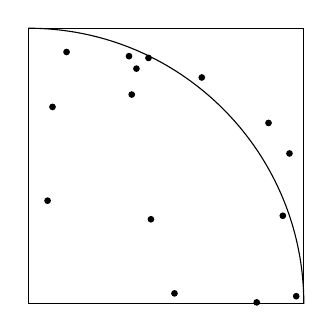
\begin{tikzpicture}[scale = 3.5]
\draw (0, 0) -- (1, 0) -- (1, 1) -- (0, 1) -- (0, 0);
\draw (1, 0) arc(0 : 90 : 1);
\foreach \x/\y in{0.87191285703751/0.6563122432321153, 
                 0.5306959423795037/0.0378441684619073, 
                 0.3926424910208062/0.8534399374103802, 
                 0.8290528045972527/0.0051887911786343555, 
                 0.44523987420676614/0.306773767907328, 
                 0.36571421038583707/0.8985764801225241, 
                 0.0880415771413442/0.7144957506587118, 
                 0.9238688817671851/0.3194878437031575, 
                 0.43641679290302626/0.8922435816528306, 
                 0.37558905614526916/0.7593054077827674, 
                 0.6297702539550359/0.8212679420429494, 
                 0.9479414508686345/0.5455882981536011, 
                 0.13907166966697593/0.9137945821304073,
                 0.9724067031078623/0.027609979517418393, 
                 0.0702349135242013/0.3743199879518039}
    \draw[fill] (\x, \y) circle(0.01);
\end{tikzpicture}
\end{center}
\end{minipage}
%-------------------------------------------------------------------------------

Écrire une fonction \type{approx\_pi(n)} qui utilise cette méthode pour déterminer une valeur approchée de $\pi$ en choisissant $n$ points dans le carré unité.
\end{Exercise}
%-------------------------------------------------------------------------------
\begin{Answer}
%-------------------------------------------------------------------------------
\begin{lstlisting}
from random import random

def approx_pi(n):
    dedans = 0
    for i in range(n):
        x = random()
        y = random()
        if x**2 + y**2 < 1:
            dedans = dedans + 1
    return dedans/n*4
\end{lstlisting}
%-------------------------------------------------------------------------------
\end{Answer}
%-------------------------------------------------------------------------------
\begin{lstlisting}
>>> approx_pi(1000000)
3.140632
\end{lstlisting}
%-------------------------------------------------------------------------------
%-------------------------------------------------------------------------------
\begin{Exercise}[title= Triangles rectangles]
On cherche les triangles rectangles dont les longueurs des cotés sont des entiers. 

Plus précisément on cherche les entiers $a$, $b$ et $c$ tels que $a\le b$ et $a^2+b^2=c^2$. 

On dit que $(a,b,c)$ est un {\bf triplet pythagoricien}.

Écrire une fonction \type{pythagoriciens(n)} qui renvoie le nombre de triplets pythagoriciens $(a,b,c)$ avec $1\le a \le n$, $1\le b \le n$ et $1\le c \le n$.

Il y a 20 solutions pour $n=50$, 127 pour $n=200$ et 881 pour $n=1000$.
\end{Exercise}
%-------------------------------------------------------------------------------
\begin{Answer}
\begin{lstlisting}
def pythagoriciens(n):
    nombre = 0
    for a in range(1, n+1):
        for b in range(i, n+1):
            for c in range(j, n+1):
                if a**2 + b**2 == c**2:
                    nombre = nombre + 1
    return nombre
\end{lstlisting}

Pour $n=1000$, ce programme est trop lent.

On peut obtenir la valeur avec 
\begin{lstlisting}
def pythagoriciens1(n):
    nombre = 0
    for a in range(1, n+1):
        for b in range(a, n+1):
            r = (a**2 + b**2)**0.5
            if r == int(r) and r <= n:
                    nombre = nombre + 1
    return nombre
\end{lstlisting}
\newpage
\end{Answer}
%-------------------------------------------------------------------------------
%Euler 19 (solution 171)
%-------------------------------------------------------------------------------
%-------------------------------------------------------------------------------
\begin{Exercise}[title= Suite $3n+1$ ]
On définit une suite $(u_n)_{n\in \N}$ par son premier terme $p$ et par la relation
\[u_{n+1} = \left\{\begin{matrix} u_n/2&\text{si $n$ est pair}\\
3u_n+1&\text{si $n$ est impair}\end{matrix}\right.\]
Écrire une fonction \type{suite(u0, n)} qui calcule $u_n$.
\end{Exercise}
%-------------------------------------------------------------------------------
\begin{Answer}
\begin{lstlisting}
def suite(u0, n):
    u = u0
    for i in range(n):
        if n%2 == 0!
            u = u//2
        else:
            u = 3*u + 1
    return u
\end{lstlisting}
\end{Answer}
%-------------------------------------------------------------------------------
%-------------------------------------------------------------------------------
\begin{Exercise}[title= PGCD]
Proposer une fonction \type{pgcd(n, p)} qui détermine le plus grand diviseur commun de $n$ et $p$ entiers positifs, c'est-à-dire le plus grand entier qui divise $n$ et $p$. Il est compris entre 1 et \type{min(n, p)}.
\end{Exercise}
%-------------------------------------------------------------------------------
\begin{Answer}
\begin{lstlisting}
def pgcd(a,b):
    commun = 1
    for k in range(1, min(a,b)+1):
        if (a % k == 0) and (b % k == 0 ):
            commun = k
    return commun
\end{lstlisting}
\end{Answer}
%-------------------------------------------------------------------------------
%-------------------------------------------------------------------------------
\begin{Exercise}[title= Nombres premiers]

Un entier $n\ge 2$ est {\bf premier} s'il n'admet pas d'autre diviseur que 1 et lui-même.

On rappelle qu'un entier est premier si et seulement si il n'admet aucun diviseur entre 2 et $\lfloor\sqrt n\rfloor$.

Écrire une fonction \type{estPremier(n)} qui renvoie \type{True} et \type{False} selon que $n$ est premier ou non.
\end{Exercise}
%-------------------------------------------------------------------------------
\begin{Answer}
\begin{lstlisting}
def estPremier(n):
    max = int(n**0.5)
    for k in range(2, max+1):
        if n%k == 0:
            return False
    return True
\end{lstlisting}
\end{Answer}
%-------------------------------------------------------------------------------
%-------------------------------------------------------------------------------
\begin{Exercise}[title= Conjecture de Golbach]
Écrire une fonction \type{goldbach(n)} qui retourne un couple de nombres premiers $(a,b)$ tels que $a+b=n$ lorsque $n$ pair.

Exemple : \type{goldbach(232) -> (3, 229)} et \type{goldbach(252) -> (11, 241)}.

On peut exclure les cas où $n$ est impair avec l'instruction
\begin{lstlisting}
assert(n%2 == 0)
\end{lstlisting}
\end{Exercise}
%-------------------------------------------------------------------------------
\begin{Answer}
\begin{lstlisting}
def goldbach(n):
    assert(n%2 == 0)
    for k in range(2, n//2+1):
        if estPremier(k) and estPremier(n-k):
            return (k, n-k)
\end{lstlisting}
\end{Answer}

%-------------------------------------------------------------------------------
\newpage
%-------------------------------------------------------------------------------
\section{Compléments}
%-------------------------------------------------------------------------------
%-------------------------------------------------------------------------------
\subsection{Bataille navale}
%-------------------------------------------------------------------------------
%-------------------------------------------------------------------------------
On considère un jeu de bataille navale simplifié : il ne s'agit pas de couler le porte-avions mais plutôt une barque tenant sur une seule case repérée par ses coordonnées \type{ligne0} et \type{colonne0} qui sont des variables globales. On fait un tir sur une case repérée par ses coordonnées \type{ligne} et \type{colonne}. On veut alors le comportement suivant :

\begin{itemize}
	\item si la barque est exactement sur la case considérée, le programme imprime le texte "{\bf Coulé}",
	\item si le tir atteint la bonne ligne ou la bonne colonne, le programme imprime "{\bf En vue}",
	\item si le tir est totalement raté, le programme imprime "{\bf À l'eau}".
\end{itemize}

On propose la fonction suivante :

\begin{lstlisting}
def bataille(ligne,colonne):
    if ligne == ligne0 or colonne == colonne0:
        print("En vue")
    elif ligne == ligne0 and colonne == colonne0:
        print("Coulé")
    else :
        print("À l'eau")
\end{lstlisting}
%-------------------------------------------------------------------------------
%-------------------------------------------------------------------------------
\begin{Exercise}[title=Correction]
%-------------------------------------------------------------------------------
Pourquoi cette fonction n'est-elle pas correcte ?

Proposer une fonction valide.
\end{Exercise}
%-------------------------------------------------------------------------------
\begin{Answer}
Si on calcule la fonction avec les bonnes coordonnées, la condition 
 
  \type{ligne == ligne0 or colonne == colonne0} va être évaluée en \type{True} donc la fonction va retourner "En vue" au lieu de "Coulé".

Il suffit d'inverser les deux premières conditions.
\begin{lstlisting}
def bataille(ligne,colonne):
    if ligne == ligne0 and colonne == colonne0:
        return "Coulé"
    elif ligne == ligne0 or colonne == colonne0:
        return "En vue"
    else :
        return "À l'eau"
\end{lstlisting}
\newpage
\end{Answer}
% %-----------------------------------------------------------------------------
% %-----------------------------------------------------------------------------
% \begin{Exercise}[title=Simplification ?]
% %-------------------------------------------------------------------------------
% Proposer une fonction qui n'utilise pas les opérateurs \type{and} et \type{or}.
% \end{Exercise}
% %-----------------------------------------------------------------------------
% \begin{Answer}
% On peut imbriquer les conditions.
% \begin{lstlisting}
% def bataille(ligne,colonne):
%     if ligne == ligne0:
%         if colonne == colonne0:
%             return "Coulé"
%         else:
%             return "En vue"
%     else:
%         if colonne == colonne0:
%             return "En vue"
%         else:
%             return "À l'eau"
% \end{lstlisting}
% \end{Answer}
%-------------------------------------------------------------------------------
%-------------------------------------------------------------------------------
\begin{Exercise}[title=Amélioration]
%-------------------------------------------------------------------------------
En général, à la bataille navale, un bateau n'est "en vue" que si la case visée est immédiatement voisine de celle du bateau. Modifier le programme de bataille navale afin de tenir compte de cette règle. On commencera par le cas où les cases diagonalement adjacentes de la barque sont "en vue" puis on traitera le cas où elle ne le sont pas. 
\end{Exercise}
%-------------------------------------------------------------------------------
\begin{Answer}
Si les points proches contiennent la diagonale alors ils forment un carré.
\begin{lstlisting}
def bataille2(ligne,colonne):
    if ligne == ligne0 and colonne == colonne0:
        return "Coulé"
    elif     abs(ligne - ligne0) <= 1 
         and abs(colonne - colonne0) <= 1:
        return "En vue"
    else:
        return "À l'eau"
\end{lstlisting}

Sinon il faut une égalité d'une coordonnée et un écart de 1 au plus pour l'autre donc une somme des écarts majorée par 1.
\begin{lstlisting}
def bataille2(ligne,colonne):ff
    if ligne == ligne0 and colonne == colonne0:
        return "Coulé"
    elif  (abs(ligne-ligne0) + abs(colonne-colonne0) <= 1):
        return "En vue"
    else :
        return "À l'eau"
\end{lstlisting}
\end{Answer}
%-------------------------------------------------------------------------------
%-------------------------------------------------------------------------------
\subsection{Calcul mental}
%-------------------------------------------------------------------------------
%-------------------------------------------------------------------------------
%-------------------------------------------------------------------------------
La fonction \type{randint} du module \type{random} permet de calculer un entier aléatoirement : \type{randint(1, 6)} renvoie un entier au hasard dans $\{1, 2, 3, 4, 5, 6\}$.
\begin{lstlisting}
from random import randint
\end{lstlisting}

La fonction \type{sleep} du module \type{time} engendre une pause dans le programme : \type{sleep(5)} attend 5 secondes.

\begin{lstlisting}
from time import sleep
\end{lstlisting}

Tester le programme suivant : 
\begin{lstlisting}
def addition1():
    a = randint(1,10)
    b = randint(1,10)
    print(a,'+',b,'=')
    time.sleep(4)
    return a+b
\end{lstlisting}
%-------------------------------------------------------------------------------
%-------------------------------------------------------------------------------
\begin{Exercise}[title=Opérations]
%-------------------------------------------------------------------------------
Construire une fonction \type{calculMental} qui propose de chercher au hasard une addition de nombres entiers à 3 chiffres ou un produit de nombres entiers à 2 chiffres et laisse un temps raisonnable pour la recherche de la réponse.
\end{Exercise}
%-------------------------------------------------------------------------------
\begin{Answer}
\begin{lstlisting}
from random import randint
import time

def calculMental():
    op = randint(1, 2)
    if op == 1:
        a= randint(100, 999)
        b= randint(100, 999)
        print("{} + {} = ?".format(a, b))
        time.sleep(6)
        print(a + b)
    else:
        a = randint(10, 99)
        b = (10, 99)
        print("{} * {} = ?".format(a, b))
        time.sleep(13)
        print(a*b)
\end{lstlisting}
\end{Answer} 
%-------------------------------------------------------------------------------
%-------------------------------------------------------------------------------
\begin{Exercise}[title=Un jeu]
%-------------------------------------------------------------------------------
Construire une fonction \type{challenge(n)} qui propose $n$ lancements successifs de \type{calculMental}.
\end{Exercise}
%-------------------------------------------------------------------------------
\begin{Answer}
\begin{lstlisting}
def challenge(n):
    for i in range(n):
    calculMental()
\end{lstlisting}
\end{Answer} 
%-------------------------------------------------------------------------------
%-------------------------------------------------------------------------------
% \begin{Exercise}[title={Entrée-sortie}]
% \begin{enumerate}
% \item Commenter les instructions suivantes et leur résultats (obtenus dans la console).
% \begin{lstlisting}[frame=lines]
% >>> a=input()
% 4
% >>> type(a)
% <class 'str'>
% >>> b=int(a)
% >>> type(b)
% <class 'int'>
% >>> 
% \end{lstlisting}
% \item Modifier \type{calculMental} en utilisant \type{input} pour faire entrer la réponse par l'utilisateur, la machine dira si c'est correct ou non ou si le temps est dépassé. Modifier aussi la fonction \type{challenge } afin qu'elle renvoie le pourcentage de réussite.
% \end{enumerate}

% \end{Exercise}
% %-------------------------------------------------------------------------------
% \begin{Answer}
%  \begin{lstlisting}
% def calculMentalbis():
%     op = randint(1,2)
%     if op==1:
%         a= randint(100, 999)
%         b= randint(100, 999)
%         print("{} + {} = ?".format(a, b))
%         delai = 6
%         resultat = a + b
%     else:
%         a=random.randint(9,99)
%         b=random.randint(9,99)
%         print(a,'*',b,'=')
%         delai = 13
%         resultat = a * b
%     t = time.time()
%     res = input("Taper votre reponse avant {} secondes".format(delai))
%     res = int(res)
%     dt = time.time()-t
%     if res == resultat and dt <= delai:
%         print('Bravo')
%     elif dt > delai and res == resultat:
%         print('Vous avez depasse le temps imparti mais le resultat est correct')
%     else: 
%         print("La bonne réponse est {}".format(resultat))
% \end{lstlisting}
% \end{Answer} 

% \begin{Exercise}[title={Analyser des structures conditionnelles}]
% % Utile ???
% Plusieurs fonctions ont pour vocation de regarder si un nombre est divisible par 2 ou par 3 (division euclidienne).
% Indiquer quelle est la valeur renvoyée par les fonction en \type{20}, \type{12}, \type{105} et \type{7}.

% Que peut-on en conclure ?

% \begin{multicols}{3}
% \setlength{\columnseprule}{1pt}

% \begin{lstlisting}[frame=no]
% def f1(a):
%     if a%2 == 0:
%         b = 2
%     if a%3 == 0:
%         b = 3
%     return b
% \end{lstlisting}

% \columnbreak %il faut ensuite passer une ligne

% \begin{lstlisting}[frame=no]
% def f2(a):
%     if a%2 == 0:
%         b = 2
%     if a%3 == 0:
%         b = 3
%     else:
%         b = 0
%     return b
% \end{lstlisting}

% \columnbreak %il faut ensuite passer une ligne

% \begin{lstlisting}[frame=no]
% def f3(a):
%     if a%2 == 0:
%         b = 2
%     elif a%3 == 0:
%         b = 3
%     else:
%         b = 0
%     return b
% \end{lstlisting}
% \end{multicols}
% \begin{multicols}{3}
% \setlength{\columnseprule}{1pt}

% \begin{lstlisting}[frame=no]
% def f4(a):
%     if a%2 == 0:
%         return 2
%     if a%3 == 0:
%         return 3
%     return 0
% \end{lstlisting}

% \columnbreak %il faut ensuite passer une ligne

% \begin{lstlisting}[frame=no]
% def f5(a):
%     if a%2 == 0:
%         return 2
%     elif a%3 == 0:
%         return 3
%     return 0
% \end{lstlisting}

% \columnbreak %il faut ensuite passer une ligne

% \begin{lstlisting}[frame=no]
% def f6(a):
%     if a%3 == 0:
%         b = 3
%     elif a%2 == 0:
%         b = 2
%     else:
%         b = 0
%     return b
% \end{lstlisting}
% \end{multicols}
% \end{Exercise}
% %-------------------------------------------------------------------------------
% \begin{Answer}
% \begin{center}
% \begin{tabular}{c|cccccc}
%   \type{a}&\type{f1(a)}&\type{f2(a)}&\type{f3(a)}&\type{f4(a)}&\type{f5(a)}&\type{f6(a)}\\
%   \hline
%   20&2&0&2&2&2&2 \\
%   12&3&3&2&2&2&3 \\
%   105&3&3&3&3&3&3\\
%   7&\color{red}{error}&0&0&0&0&0\\
% \end{tabular}
% \end{center}

% Il vaut mieux éviter de faire des fonctions qui devraient répondre à plusieurs questions.
% \end{Answer}
